\documentclass[12pt, a4paper]{article} 
%\documentclass[12pt, a4paper, twoside]{article} twoside bewirkt ,d ass %Zweiseitenformat angezeigt wird !
%ohne Draft werden die Bilder mitcompiliert // \documentclass[12pt, a4paper, draft]
\usepackage[german]{babel}
\usepackage[latin1]{inputenc}
\usepackage{graphicx, color}
	\DeclareGraphicsExtensions{.png}
	\graphicspath{{Figures/}}
\usepackage[pdftex,
						colorlinks, linkcolor=blue, urlcolor=blue,
						bookmarks=true,									   %%% es werden Bookmarks erzeugt
						bookmarksopen=false,  							 %%% Bookmarks werden alle angezeigt
						bookmarksnumbered=true]            %%% ... with numbers
					  {hyperref}
\usepackage[all]{hypcap}
\usepackage{wsp}

% die Titelseite f�r den Plotter

\bcetitlepage
{
	Dr. Dagmar Bley, Gernot Belger
}
{
	Stand \today
}
{\wspplot}
{
		Ein Programm zur Erzeugung von \\
		L�ngs- und Querprofilzeichnungen
}
{
	2.0
}

\pagestyle{headings}
%\makeindex

\begin{document}


	
%Titelseite
\maketitle
\thispagestyle{empty}
\clearpage


% Inhaltsverzeichnis
\hypertarget{toc}{}
\tableofcontents

% die einzelnen Sections
% Die Einfuehrung fuer das PlotterHandbuch

\section{Einf�hrung}

\wspplot\ ist ein Programm zur Erzeugung von L�ngs- und
Querprofilzeichnungen im Rahmen der Spiegellinienberechnung. Die
Dateiverwaltung ist analog zu \wspwin\ aufgebaut und in Projekte, Zust�nde
und Profile gegliedert. Es k�nnen L�ngs- und Querprofile im
\wspwin-Format f�r den Plot aufbereitet werden. Das Programm umfa�t
s�mtliche Ge\-staltungs\-m�glich\-keiten der Zeichnung bis hin zum
eigentlichen Ausdruck auf Papier. Ein zus�tzliches CAD-Programm ist
nicht erforderlich, wenngleich eine DXF-Schnittstelle zum
Datenaustausch mit CAD-Programmen integriert ist. Trotz der
umfangreichen M�glichkeiten zur Aufbereitung der Plots, die
\wspplot\ bietet, ist die Programmkonzeption sehr einfach. Fast
alle Funktionen lassen sich �ber den Men�punkt \menu{Bearbeiten / Eigenschaften} aufrufen.


\section{Projektverwaltung}

\subsection{Begriffserl�uterung}
Die Projektverwaltung verl�uft analog der bew�hrten Struktur im BCE-Spiegel\-linien\-pro\-gramm
\wspwin\ und gliedert sich in:\\

\begin{itemize}
	\item {\textbf{Projekt:}}
	ein benutzerdefiniertes Verzeichnis, in dem alle Daten, die in einem
	inhaltlichen Zusammenhang zueinander stehen, abgelegt sind (z.B. alle Daten
	im Einzugsgebiet des Neckars).
	
	\item {\textbf{Gew�sser:}}
	innerhalb eines Projektes k�nnen mehrere Gew�sser (z.B. aus demselben
	Einzugsgebiet) definiert werden
	
	\item {\textbf{Zustand:}}
	f�r jedes Gew�sser k�nnen schlie�lich mehrere geometrische Zust�nde (z.B.
	Ist-Zustand, Planungsfall) angelegt werden. Innerhalb eines Zustandes
	existieren schlie�lich Quer- und L�ngsprofile, die die notwedigen 
	Informationen beinhalten.
	
	\item {\textbf{Abfl�sse:}}
	Es k�nnen mehrere Abflussereignisse verarbeitet werden.
	
	\item {\textbf{Varianten:}}
	unterschiedliche Eingaben f�r die hydraulische Berechnung werden in
	Berechnungsvarianten organisiert.
	
\end{itemize}

\hypertarget{cmd:beenden}{}
\hypertarget{cmd:datei-projektmanager}{}
\subsection{Projektmanager}
\subsubsection{Allgemeines}

Bevor mit \wspmap\ gearbeitet werden kann, m�ssen Projekte, Zust�nde und 
Querprofile angelegt sein. Die Projektverwaltung erfolgt
(wenn nicht bereits Projekte aus \wspwin\  vorhanden sind) komplett �ber den Projektmanager, der aus dem Men� \\ \menu{Datei / Projektmanager} ge�ffnet wird
(�ffnet sich bei Programmstart automatisch)(siehe Abb. \ref{fig:menu_pm} und \ref{fig:projektmanager}). 

\begin{figure}[hbtp]
	\begin{center}
		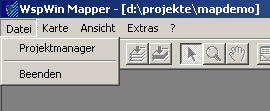
\includegraphics[scale=0.70]{abb1}
	\end{center}
	\caption{Projektmanager �ffnen}
	\label{fig:menu_pm}
\end{figure}

�ber den Men�punkt \menu{Projekt / Neu} im Projektmanager wird ein neues
Projekt angelegt. Dazu muss der entsprechende Pfad eingegeben oder ausgew�hlt werden (z.B. \file{D:/projekte/bfg/rhein}. 

Falls bereits Projekte existieren, die aber nicht in der Liste aufgef�hrt sind, k�nnen diese 
�ber \menu{Einf�gen} importiert werden)(Abb. \ref{fig:projektmanager}).

\begin{figure}[hbtp]
	\begin{center}
		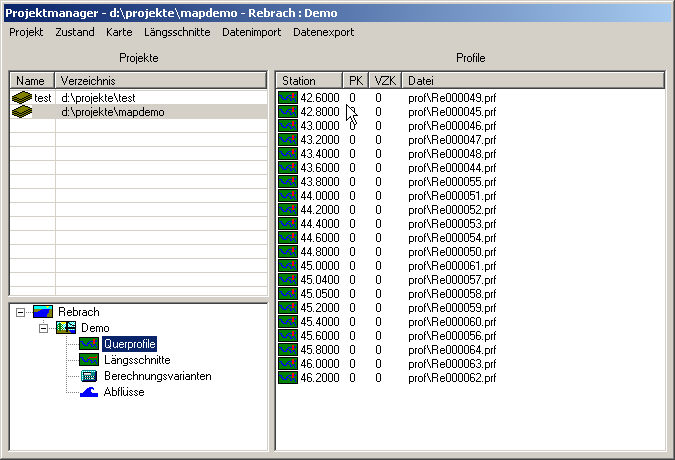
\includegraphics[scale=0.65]{abb2}
	\end{center}
	\caption{Projektmanager}
	\label{fig:projektmanager}
\end{figure}

Bei Auswahl eines der aufgef�hrten Projekte werden s�mtliche Gew�sser und die dazugeh�rigen Zust�nde eines Projektes, sofern bereits Daten vorhanden sind, angezeigt. Wenn noch keine Daten
existieren, muss zun�chst ein neuer Zustand �ber den Men�punkt \menu{Zustand / Neu} definiert werden. In der
daraufhin erscheinenden Maske wird der Gew�ssername und eine
Zustandsbezeichnung eingegeben. Es k�nnen mehrere Zust�nde f�r dasselbe Gew�sser angelegt werden. Nachdem Sie einen neuen Zustand angelegt haben, wird
dieser in der �bersicht aufgef�hrt. Durch Aktivierung des +/- K�stchens k�nnen Sie ein
Gew�sser bzw. einen Zustand in der Baumstruktur aufklappen, woraufhin Querprofile,
L�ngsschnitte, Abfl�sse und Berechnungsvarianten zur Auswahl stehen.

\subsubsection{Datenimport}
Bez�glich des Datenimports stehen unabh�ngig von \wspwin\  verschiedene Schnitt\-stel\-len zum Datenimport zur Verf�gung.\\

Weitere Beschreibungen und Beispieldateien zu den oben genannten Import-Formaten befinden sich auf
der WspWin-CD im Verzeichnis \menu{Informationen/Import-Export-Formate}. 

Folgende Datenformate werden unterst�tzt:\\

\underline{Geometrische Daten:}

\begin{itemize}
	\item {DA66:}
	Profilgeometrie gem. REB-Standard
	\item {DA50:}
	Georeferenzierung der Profilfestpunkte
	\item {WSV:}
	Standardformat der Wasser- und Schiffahrtsverwaltung
	\item {Tripple:}
	Fluss-km, x-Koordinate, y-Koordinate, z-Koordinate, ggf. \\
	Kennung (jeweils durch	Kommata getrennt)
\end{itemize}

Beim Import von DA66-Dateien ist die Reihenfolge zu be\-achten (zuerst DA66 und dann die
Georeferenzierung in DA50). Sollten die Daten in einer Datei vorliegen, ist diese 2x (einmal
�ber DA66 und einmal �ber den Men�punkt DA50) zu importieren.
\\
Bei Import des Tripple-Formats k�nnen Knickpunkte durch zus�tzliche Eingabe der Kennung
KP hinter der letzten Koordinaten gekennzeichnet werden. Die Abst�nde innerhalb des Profils
(y-Koordinaten) berechnen sich aus der Distanz zum ersten Profilpunkt bzw. zum zuletzt gelesenen Knickpunkt.
Ebenso kann die Lage der Trennfl�chen durch die Kennzeichnung RU und LU markiert
werden. Die durchstr�mten Bereiche werden stets automatisch auf den letzten Knickpunkt
(bzw. den ersten Profilpunkt ) vor der ersten Trennfl�che und den ersten Knickpunkt (bzw.
letzten Profilpunkt) nach der zweiten Trennfl�che gesetzt.

\underline{Hydraulische Daten:}\\
�ber den Men�punkt \menu{Hyk} k�nnen die Lage von Durchstr�mten Bereichen, Trennfl�chen und
Modellgrenzen sowie von B�schungskanten gem�� BfG\footnote{Bundesanstalt f�r Gew�sserkunde}-Format importiert werden:\\
Bsp.:\\
RL VL HF VR RR:\\
RL  $\Rightarrow$  Modellgrenze li. Grenze\\
VL  $\Rightarrow$  Durchstr�mter Bereich li. Grenze\\
HF  $\Rightarrow$  Trennfl�che links\\
VR  $\Rightarrow$  Trennfl�che rechts\\
RR  $\Rightarrow$  Durchstr�mter Bereich rechte Grenze\\
d.h. RL-VL =Durchstr�mter Bereich links\\
VL-HF = Vorland links\\
HF-VR = Haupt�ffnung\\
VR-RR = rechtes Vorland\\

Berechnete Wasserst�nde im WST-Format der BfG k�nnen mit den zugeh�rigen Abfl�ssen �ber den Men�punkt WST importiert werden. Sie werden in Berechnungsvarianten bzw.
L�ngsschnitten gespeichert. Aus den L�ngsschnitten k�nnen die Wasserspiegel �ber die
Men�folge \\ \menu{L�ngsschnitt / Wsp einf�gen} in die Profile eingetragen werden \\ (Abb. \ref{fig:abbdrei}), damit diese als �berschwemmungsgrenzen in der Karte angezeigt werden. So k�nnen z.B.
verschiedene Abfl�sse in Berechnungsvarianten / L�ngsschnitten verwaltet werden. Ebenso
k�nnen nicht mehr ben�tigte Wasserspiegeleintr�ge wieder entfernt werden.


\begin{figure}[hbtp]
	\begin{center}
		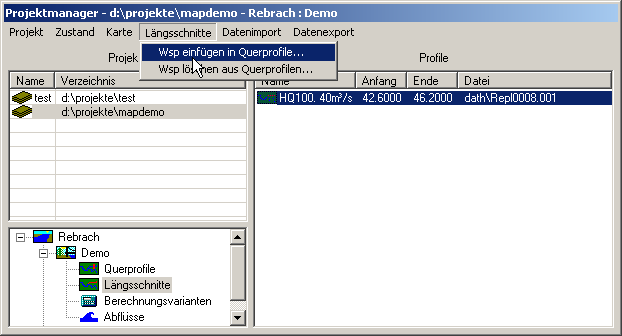
\includegraphics[scale=0.60]{abbdrei}
	\end{center}
	\caption{Men�folge: Wasserspiegel in Profile eintragen}
	\label{fig:abbdrei}
\end{figure}

Der Datenimport erfolgt stets durch Selektion einer Datei im
Standard-Windows-Dialog. Zu beachten ist, da� die importierten Daten in jedem Fall �ber
ihre Gauss-Kr�ger-Koordinaten georeferenziert sein m�ssen, um im \wspmap\ dargestellt zu
werden. Nachdem alle Daten importiert wurden, schlie�t sich das Fenster des
Projektmanagers automatisch.

\subsubsection{Datenexport}
�ber den Projektmanager k�nnen Daten (\menu{Datenexport}) nach der Bearbeitung 
in \wspmap\ auch in verschiedene oben beschriebene Formate exportiert werden.

\subsubsection{Projekt �ffnen}

Bevor mit \wspmap\ gearbeitet werden kann, mu� immer erst ein Projekt im Projektmanager ge�ffnet werden. Dies erfolgt im Projektmanager �ber den Men�\-punkt \menu{Projekt / �ffnen}.
Nachdem ein Projekt ge�ffnet wurde, wird es im Fenstertitel der Anwendung angezeigt.


\hypertarget{cmd:karte-neu}{}
\hypertarget{cmd:karte-oeffnen}{}
\hypertarget{cmd:karte-loeschen}{}
\section{Arbeiten mit Karten}
Die Arbeit mit \wspwin\ Mapper basiert auf Karten. In einer Karte werden die \wspwin\ Projektdaten im Lageplan dargestellt und bearbeitet. Jede Karte kann dabei eine beliebige Auswahl von Profilen eines Projektes beinhalten. Neben den hydraulischen Daten k�nnen in die Karten Hintergrundbilder (z.B: TK, Luftbilder) oder andere Vektordaten (Flussachsen, Uferlinien, usw.) geladen werden.

\subsection{Kartenerstellung}

Bevor mit der Bearbeitung von Daten in einem Lageplan begonnen werden kann, ist zun�chst
eine neue Karte zu erstellen (Men�folge \menu{Karte / Neu}).
Es erscheint die Aufforderung, einen Namen f�r die zu erstellende Karte zu
vergeben (bei vorhandenen \wspwin\-Projekten stehen nach einem Klick auf die
Pfeiltaste die bereits angelegten Zust�nde zur Verf�gung). Jetzt �ffnen sich
zwei neue Fenster: das eigentliche Kartenfenster und das Profil�bersichtsfenster mit den
Profilen des Projektes. 

\hypertarget{cmd:ansicht-profiluebersicht}{}
\hypertarget{cmd:karte-vorlagespeichern}{}
\subsection{Profil�bersicht}
\subsubsection{Profildaten laden und aktualisieren}
Im n�chsten Schritt der Projektbearbeitung sind die Projekt-Daten in die Karte
zu laden (Tipp: man sollte nur Daten einer Berechnungsvariante laden!). Dies erfolgt �ber das Profil�bersichtsfenster, in dem die Profile entweder einzeln durch Aktivierung des Kontrollk�stchens oder durch Mehrfachselektion in dem Listenfeld (Shift + Pfeiltaste) und anschlie�ender Bet�tigung des + oder - Knopfes hinzugeladen oder entfernt werden k�nnen (Abb. \ref{fig:abb4}). Mit dem Knopf 'A' werden alle Querprofile ausgew�hlt.

\begin{figure}[hbtp]
	\begin{center}
		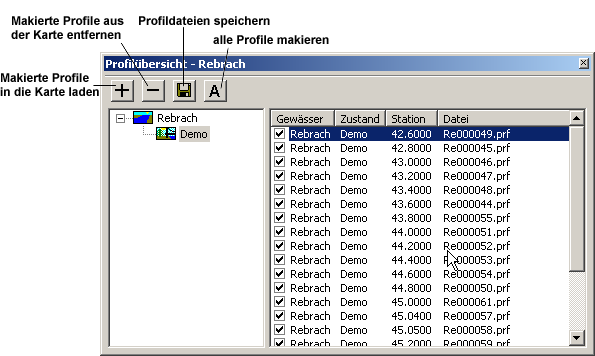
\includegraphics[scale=0.60]{abb4}
	\end{center}
	\caption{Profil�bersichtsfenster}
	\label{fig:abb4}
\end{figure}

\subsubsection{Profildaten speichern}
\label{subsec:profildaten-speichern}
In einer Karte dargestellte Profile k�nnen jederzeit durch Bet�tigung des
Speichern-Knopfes in dem Profil�bersichtsfenster (Diskettensymbol) gespeichert werden. Dazu m�ssen die zu speichernden Profile selektiert sein. (Achtung: Die vorhandenen Profildateien werden dadurch �berschrieben!)
Umgekehrt k�nnen die in der Karte dargestellten
Informationen st�ndig mit au�erhalb des Mappers (z.B. in \wspwin) ver�nderten Profilinformationen
erneuert werden. Die entsprechenden Profile sind einfach noch einmal zu laden. 
\\
Beim Aktualisieren der Informationen in den Profildateien �ber das Diskettensymbol erfolgt eine
Abfrage, welche Themen erneuert werden sollen. So l��t sich einerseits zwischen den
Datens�tzen Trennfl�chen, Durchstr�mten Bereichen und Rauheiten w�hlen; andererseits
k�nnen z.B. die Informationen aus angelegten Rauheits- oder Vegetationszonen �bernommen
werden. Wenn mehrere Wertefelder angelegt wurden (z. B. bei der Rauheit) kann schlie�lich ein entsprechender Wert
zugeordnet werden. Parameter und Werte werden dann in die Profildateien �bertragen.


%############################################################################
\hypertarget{cmd:tools-maximaledarstellung}{}
\hypertarget{cmd:tools-ausschnittvergoessern}{}
\hypertarget{cmd:tools-ausschnitverkleinern}{}
\hypertarget{cmd:tools-ausschnittverschieben}{}

\subsection{Kartenfenster}
Nach dem �ffnen einer Karte stehen dem Nutzer eine Reihe von Ansichtsfenstern zur Verf�gung.

Die meisten Ansichtsfenster k�nnen in ihrer Gr��e individuell ver�ndert oder auch an eine
beliebig Stelle verschoben werden. �ber den Men�punkt \menu{Ansicht} k�nnen die verschiedenen Fenster ein- oder ausgeblendet werden (Abb. \ref{fig:abb17}).\\

\begin{figure}[hbtp]
	\begin{center}
		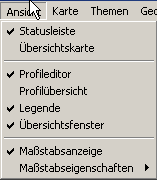
\includegraphics[scale=0.70]{abb17}
	\end{center}
	\caption{Darstellungsm�glichkeiten im Men� ANSICHT}
	\label{fig:abb17}
\end{figure}


\subsubsection{Lageplan}
Im \textbf{Kartenfenster} werden alle Projektbezogenen Daten (Querprofile, Wasserspiegel usw.) als Lageplan dargestelt. Die Reihenfolge der Darstellung wird durch die Reihenfolge der Themen in der Kartenlegende festgelegt (das Kartenfenster kann nicht ausgeblendet werden).

\hypertarget{cmd:ansicht-legende}{}
\subsubsection{Legende}
In der \textbf{Legende} werden die in das Projekt eingeladenen Themen aufgelistet.Durch Klick auf das H�kchen werden Themen ein- bzw. ausgeblendet. Zur Bearbeitung muss das entsprechende Thema makiert werden.\\(Es kann immer nur das aktive Thema bearbeitet werden.)\\Durch Rechtsklick auf ein Thema k�nnen die Men�punkte des Men�s \menu{Themen} in einem Pull-Down Men� ausgew�hlt werden. Die einzelnen Themen lassen sich nach oben oder unten verschieben, wodurch die Reihenfolge der Darstelllung definiert wird. 

\hypertarget{cmd:ansicht-uebersichtsfenster}{}
\subsubsection{�bersichtsfenster}
Im �bersichtsfenster wird die Lage des gerade aktiven (gezoomten) 
Kartenausschnitts innerhalb der Gesamtkarte durch ein
rotes K�stchen in einem separaten Fenster angezeigt(Abb. \ref{fig:abb20}).\\
Damit ein Thema im �bersichtsfenster angezeigt wird, muss es zun�chst in der Legende markiert werden und dann der Men�punkt \menu{Themen / im �bersichtsfenster anzeigen} aktiviert werden.\\

\begin{figure}[hbtp]
	\begin{center}
		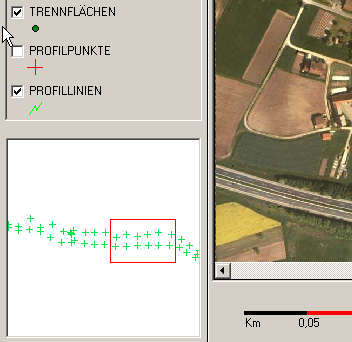
\includegraphics[scale=0.70]{abb20}
	\end{center}
	\caption{�bersichtsfenster mit Thema Wasserspiegel}
	\label{fig:abb20}
\end{figure}

\subsubsection{Profilansicht}
In der Profilansicht kann ein makiertes Profil im Querschnitt dargestellt werden.\\Zur Zeit wird nur die Darstellung des Gel�ndes sowie der Fliesszoneneinteilung (Trennfl�chen, durchst. Bereiche, B�schung) unterst�zt. Bauwerke, Durchl�sse und Rauheitsbeiwerte werden nicht dargestellt.\\Die Auswahl dws anzuzeigenden Profils wird �ber das Menu (\menu{Tools / Profilcursor}) vorgenommen.

\hypertarget{cmd:ansicht-massstabsanzeige}{}
\subsubsection{Massstabsanzeige}
Neben den zuvor erw�hnten M�glichkeiten die Darstellung zu modifizieren, besteht auch 
die M�glichkeit, �ber den Men�punkt \menu{Ansicht / Massstabsanzeige} festzulegen, ob 
eine Massstabsanzeige unter dem Kartenfenster gew�nscht wird. Die Eigenschaften die Massstabs werden im Menu \menu{Ansicht / Massstabseigenschaften} festgelegt(Abb. \ref{fig:abb21}).\\

\begin{figure}[hbtp]
	\begin{center}
		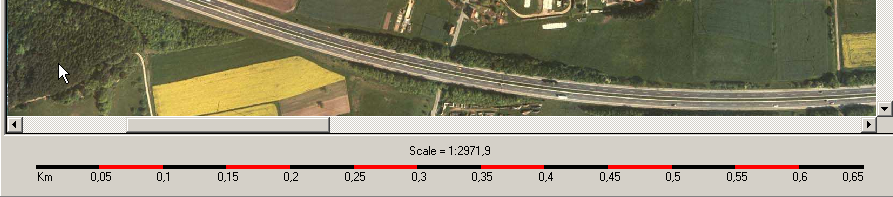
\includegraphics[scale=0.40]{abb21}
	\end{center}
	\caption{Ma�stabsanzeige in km}
	\label{fig:abb21}
\end{figure}

\subsubsection{Statuszeile}
In der Statuszeile am unteren Rand des Programmfensters werden das gerade aktive Thema, sowie die Gauss-Kr�ger-Koordinaten der aktuellen Cursorposition angezeigt.\\Daneben wird f�r jeden Men�punkt bzw. jeden Knopf der Werkzeugleiste eine Kurzbeschreibung angezeigt, sobald mit der Maus die entsprechend Funktion ausgew�hlt wird.\\bei zeitintensiven Pperationen wird hier ein Balken mit dem aktuellen Fortschritt angezeigt.

\hypertarget{cmd:ansicht-uebersichtskarte}{}
\subsubsection{�bersichtskarte}
In der \textbf{�bersichtskarte} werden in der unteren Anzeige alle im Projekt vorhandenen Karten aufgelistet.\\
Sind in einem Projekt mehrere Karten vorhanden, z.B. f�r verschiedene Gew�sser eines
Einzugsgebietes, so zeigt die �bersichtskarte automatisch die Lage der einzelnen Karten
zueinander an.\\

\subsection{Kartennavigation}
F�r die Navigation in der Karte stehen drei Werkzeuge zur Verf�gung, welche �ber die Smybolleiste (Abb. \ref{fig:abb18}) oder das Men� \menu{Tools} aktiviert werden k�nnen.

\begin{figure}[hbtp]
	\begin{center}
		
\includegraphics[scale=0.50]{abb18}
	\end{center}
	\caption{Symbolleiste}
	\label{fig:abb18}
\end{figure}


\paragraph{Maximale Darstellung (\menu{Tools / Maximale Darstellung})}
\ \\Der Kartenausschnitt wird so gew�hlt, dass alle verf�gbaren Informationen angezeigt werden.

\paragraph{Zoom zum aktiven Thema (\menu{Theman / Zoom zum aktiven Thema})}
\ \\Der Kartenausschnitt wird auf die Ausdehnung des aktiven Themas gesetzt.

\paragraph{Ausschnitt vergr��ern (\menu{Tools / Ausschnit vergr�ssern})}
\ \\�ber die Lupe kann ein beliebiger Kartenausschnitt durch Markieren eines Bereiches vergr��ert werden. Bei Klick mit der rechten Maustaste wird die Darstellung wieder verkleinert.

\subsubsection{Navigation mit der Maus}
Neben den eben beschriebenen Werkzeugen kann in der Karte mit der rechten Maustaste navigiert werden.

\begin{itemize}
	\item Ein einfacher Klick mit der rechten Taste vekleinert den dargestellten Ausschnitt (Zoom out).
	\item Mit Klicken und Festhalten der rechten Maustaste (Drag'n'Drop) kann der dargestellte Kartenausschnitt verschoben werden.
	\item Mit dem Mausrad wird der Ausschnitt der Karte jeweils vergr�ssert bzw. verkleinert (Zoom out/Zoom in).
\end{itemize}

Die Navigation mit der rechten Maustaste steht w�hrend der meisten Bearbeitungsschritte zur Verf�gung. Da die meisten Arbeitsschritte mit der linken Maustaste durchgef�hrt werden.

\hypertarget{cmd:tools-profileditieren}{}
\hypertarget{cmd:tools-profileditorautomatik}{}
\hypertarget{cmd:ansicht-profileditor}{}
\subsubsection{Kommunikation mit \wspwin\ / Querprofildarstellung}
\paragraph{Profil ansehen/editieren (\menu{Tools / Profil editieren})}
\ \\ \wspmap\ beinhaltet die M�glichkeit, im Kartenfenster parallel zur Karte ein angew�hltes Querprofil darstellen zu lassen. Hierzu w�hlt man das entsprechende Symbol bzw. die Men�folge \menu{Tools / Profil editieren} und klickt \textbf{einmal} in der Karte auf das gew�nschte Profil (das Profil wird farbig markiert). Es �ffnet
sich die Profilansicht mit dem ausgew�hlten Profil. Ein Doppelklick �ffnet \wspwin\ mit dem entsprechenden Querprofil. Im Gegensatz zur Profilansicht, das nur der Darstellung, nicht aber der Dateneingabe dient, kann das Profil in \wspwin\ auch modifiziert werden. Werden im Kartenfenster allerdings Ver�nderungen vorgenommen (z.B. Trennfl�chen verschoben), zeigt die Profilansicht direkt die Auswirkungen
im Querprofil. Die Anzeige im \wspwin\ Grafik - Editor �bernimmt diese �nderung erst nach Speicherung der Profildatenin der Profil�bersicht. 

\begin{figure}[hbtp]
	\begin{center}
		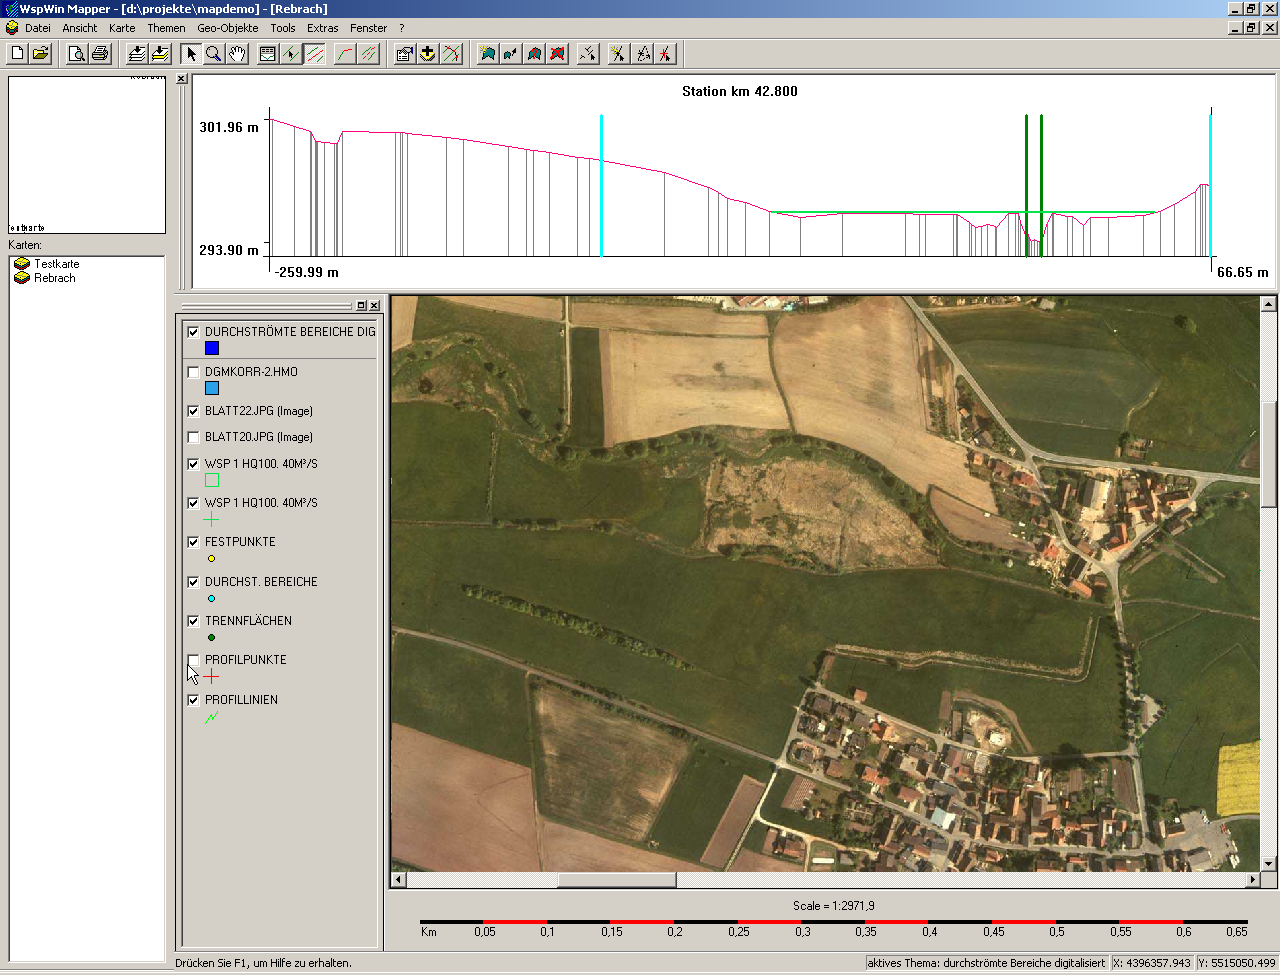
\includegraphics[scale=0.20]{abb19}
	\end{center}
	\caption{Karte mit Profileditor}
	\label{fig:abb19}
\end{figure}

\paragraph{Profileditor automatik (F5)} \menu{Tools / Profileditor Automatik}
\ \\Ist die Profileditor-Automatik aktiviert, wird die Profildarstellung mit der Maus synchronisert. D.h. n�hert sich die Maus einem Profil im Lageplan, wird dieses automatisch aktiviert und in der Profilansicht dargestellt.\\Diese Funktion kann auch �ber die F5 Taste ein- oder ausgeschaltet werden.

\paragraph{Profilcursor (F6)} \menu{Tools / Profilcursor (F6)}
\\Ist der Profilcursor aktiviert, wird die Mausposition im Lageplan als Markierung in der Profilansicht eingeblendet. Die Position der Maus wird dabei senkrecht auf das Querprofil projiziert. Zus�tzlich zur Markierung wird die H�he und Breite des markierten Punktes im lokalen Bezugssystem ausgegeben.\\
Wird der Profilcursor deaktiviert, wird die letzte Position des Cursors in der Profilansicht beibehalten.
\section{Themen bearbeiten}
\hypertarget{cmd:themen-kopieren}{}
\hypertarget{cmd:themen-zoomzumthema}{}

\hypertarget{cmd:themen-neu}{}
\subsection{Thema erzeugen}
\label{subsec:thema-erzeugen}
Das Programm kann zur aktiven Datenneueingabe genutzt werden, indem
�ber \menu{Thema / Neu} ein neues Shape-File erzeugt wird \\
(Abb. \ref{fig:abb8}).\\


\begin{figure}[hbtp]
	\begin{center}
		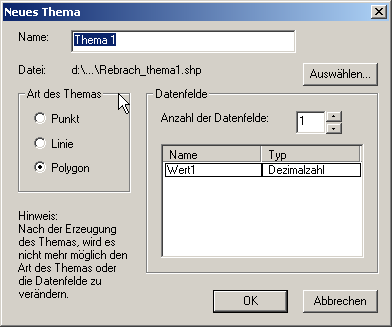
\includegraphics[scale=0.70]{abb8}
	\end{center}
	\caption{Erzeugen eines neuen Themas}
	\label{fig:abb8}
\end{figure}

%Abb.8: Erzeugung eines neuen Themas\\
Es ist zun�chst ein Name f�r das neue Thema zu vergeben, der beliebig gew�hlt
werden kann. Im n�chsten Schritt ist festzulegen, ob man ein Punkt-, Linien- oder Polygon-Shape
erzeugen m�chte. Soll das Thema beispielsweise als Trennfl�chendatensatz genutzt werden, empfiehlt es sich, ein Linien-shape anzulegen. Sobald man die Maske mit OK best�tigt hat, wird das neue Thema
(noch ohne Inhalt) in der Themen�bersicht mit aufgef�hrt. 
Zu beachten ist die Festlegung der Attribut-Datens�tze des Themas. Diese k�nnen nur beim Erzeugen eines neuen Themas festgelegt werden. Im weiteren Verlauf der Bearbeitung ist lediglich die �nderung der Werte in den Attributfeldern m�glich, nicht aber das Hinzuf�gen oder Entfernen bestimmter Attribute. 
Ein Beispiel f�r ein neues Thema ist ein Polygon-Shape, mit dem Bewuchszonen dargestellt werden k�nnen. In diesem Fall w�rde man z.B. ein Datenfeld f�r die unterschiedlichen Bewuchsklassen  anlegen (Name 'Bewuchs') anlegen und f�r den 
Datentyp 'Dezimalzahl' aus dem Listenfeld w�hlen. Im n�chsten Schritt kann nun das
erzeugte Thema bearbeitet werden (Hinzuf�gen von Elementen und Attributen; vgl. Kap.5).

\hypertarget{cmd:themen-hinzufuegen}{}
\subsection{Thema einf�gen}
\label{subsec:thema-einfuegen}
Neben importierten Daten aus \wspwin\ bietet \wspmap\ die M�glichkeit zus�tzliche Datens�tze als Themen einzuf�gen. Neben shape-Dateien und ArcInfo-Coverages
k�nnen verschiedene Raster (Image)- und Vektordaten sowie CAD-Formate eingeladen
werden, die bei Aktivierung des entsprechenden Sammel-Listeneintrags automatisch angezeigt werden.
\\
Um einen Datensatz hinzuzuf�gen, w�hlt man den Men�punkt \menu{Themen / Themen hinzuf�gen}. Hier k�nnen neben dem entsprechenden Verzeichnis auch die gew�nschten Dateiformate gew�hlt werden(Abb. \ref{fig:abb5}). Auf diese Weise k�nnen Hintergrundbilder mit den Projektdaten �berlagert werden. S�mtliche hydraulischen und geometrischen Daten werden in Form einzelner Themen entweder als Punkt (z.B. Trennfl�chen, Durchstr�mte Bereiche) oder Linien-shapes (z.B. Profillinie) dargestellt. Jeder einzelne Profilpunkt wird durch ein Kreuz markiert. Alle
Themen sind in einer �bersicht aufgef�hrt und k�nnen hier durch Anklicken f�r weitere Bearbeitungen markiert werden. 


\begin{figure}[hbtp]
	\begin{center}
		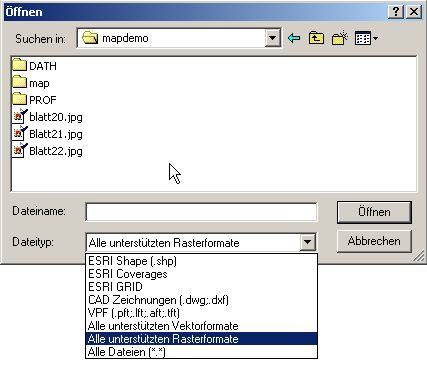
\includegraphics[scale=0.70]{abb5}
	\end{center}
	\caption{Thema aus Standard-Bildformaten hinzu laden}
	\label{fig:abb5}
\end{figure}
%Abb.5: Thema aus Standard-Bildformaten hinzu laden\\



\hypertarget{cmd:themen-verschieben-nachoben}{}
\hypertarget{cmd:themen-verschieben-einshoch}{}
\hypertarget{cmd:themen-verschieben-einsrunter}{}
\hypertarget{cmd:themen-verschieben-nachunten}{}
\hypertarget{cmd:themen-wasserspiegelnachaussen}{}
\subsection{Thema verschieben}
Nachdem ein Thema markiert wurde, kann es �ber die Men�option \menu{Thema verschieben} in der Hierarchie der Darstellung verschoben werden (z.B. wenn die Hintergrundbilder �ber statt hinter den Profilinformationen liegen). Dies ist allerdings auch durch Verschieben mit Hilfe des Mauszeigers (linke Maustaste gedr�ckt halten) m�glich (Abb. \ref{fig:abb6}).


\begin{figure}[hbtp]
	\begin{center}
		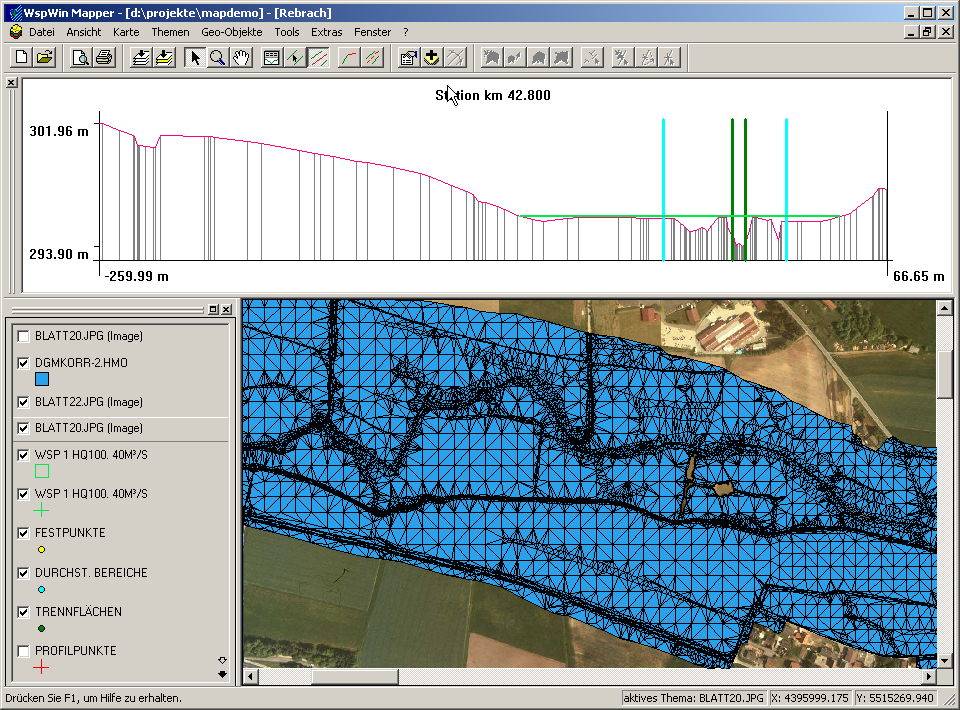
\includegraphics[scale=0.40]{abb6}
	\end{center}
	\caption{Hintergrundbilder und verschiedene Profilinformationen als Themen einer Karte}
	\label{fig:abb6}
\end{figure}
%Abb.6: Hintergrundbilder und verschiedene Profilinformationen als Themen einer Karte

\hypertarget{cmd:themen-uebersichtsfenster}{}
\hypertarget{cmd:themen-eigenschaften}{}
\subsection{Themeneigenschaften anzeigen und ver�ndern}
�ber die Men�folge \menu{Themen / Themeneigenschaften} oder alternativ durch
Doppelklick auf das Thema kann die Darstellungsweise eines Datensatzes ver�ndert
werden (Abb. \ref{fig:abb7}).\\
So l��t sich die Kartendarstellung hinsichtlich Farbe, Punktgr��e bzw. Linienst�rke oder
Symbol ver�ndern. Jedem Geoobjekt eines Themas kann ein Label (z.B. Stationierung,
Zustand, Dateiname) durch Aktivierung des Listenknopfes 'Textfeld' nach Auswahl einer
Lableart zugeordnet werden, das seinerseits wiederum umfangreich formatiert werden kann.

\begin{figure}[hbtp]
	\begin{center}
		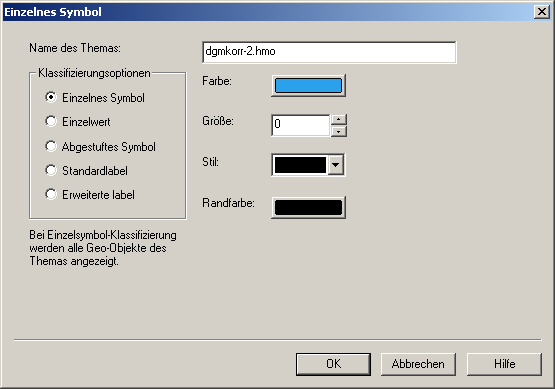
\includegraphics[scale=0.60]{abb7}
	\end{center}
	\caption{Ver�ndern von Themeneigenschaften}
	\label{fig:abb7}
\end{figure}

%Abb.7: Ver�ndern von Themeneigenschaften\\


\subsubsection{Eigenschaften importieren und exportieren}
Um h�ufiger verwendete Themeneigenschaften nicht immer wieder von Hand einzugeben ist es m�glich die Eigenschaften eines Themas in eine externe Datei zu speichern. Nach Wahl des Men�s \menu{Themen / Eigenschaften exportieren} werden die aktuellen Einstellungen in die vom Benutzer gew�hlte Datei gespeichert. Diese kann zu einem sp�teren Zeitpunkt �ber den Men�punkt �ber \menu{Themen / Einstellungen importieren} wieder geladen werden und setzt dadurch die Eigenschaften des gerade aktiven Themas.

\hypertarget{cmd:themen-entfernen}{}
\subsection{Thema entfernen}
Um dargestellte Datens�tze zu entfernen, ist der Men�punkt (\menu{Thema entfernen}) zu w�hlen. 
Soll das Thema weiterhin aufgelistet bleiben, aber nur aus der Kartendarstellung entfernt werden, ist das entsprechende Kontrollk�stchen in der Themenauflistung zu deaktivieren.\\

\subsection{Themen exportieren}
\wspmap\ legt im Projektverzeichnis auf der Festplatte ein Unterverzeichnis 'map' an. Hier
werden alle Informationen aus \wspmap\ abgelegt, u.a. auch alle themenbezogenen
Informationen. So wird f�r jedes Thema bzw. jeden Datensatz (Durchstr�mte Bereiche, Trennfl�chen, Profilpunkte...) eine shape-Datei (*.shp) angelegt, die auch in anderen Programmen (z.B. ArcView) genutzt werden kann. Zus�tzlich werden die Attribute in einer dbf-Datei gespeichet, die z.B. in das Programm Excel eingelesen und dort bearbeitet werden kann.\\

\begin{figure}[hbtp]
	\begin{center}
		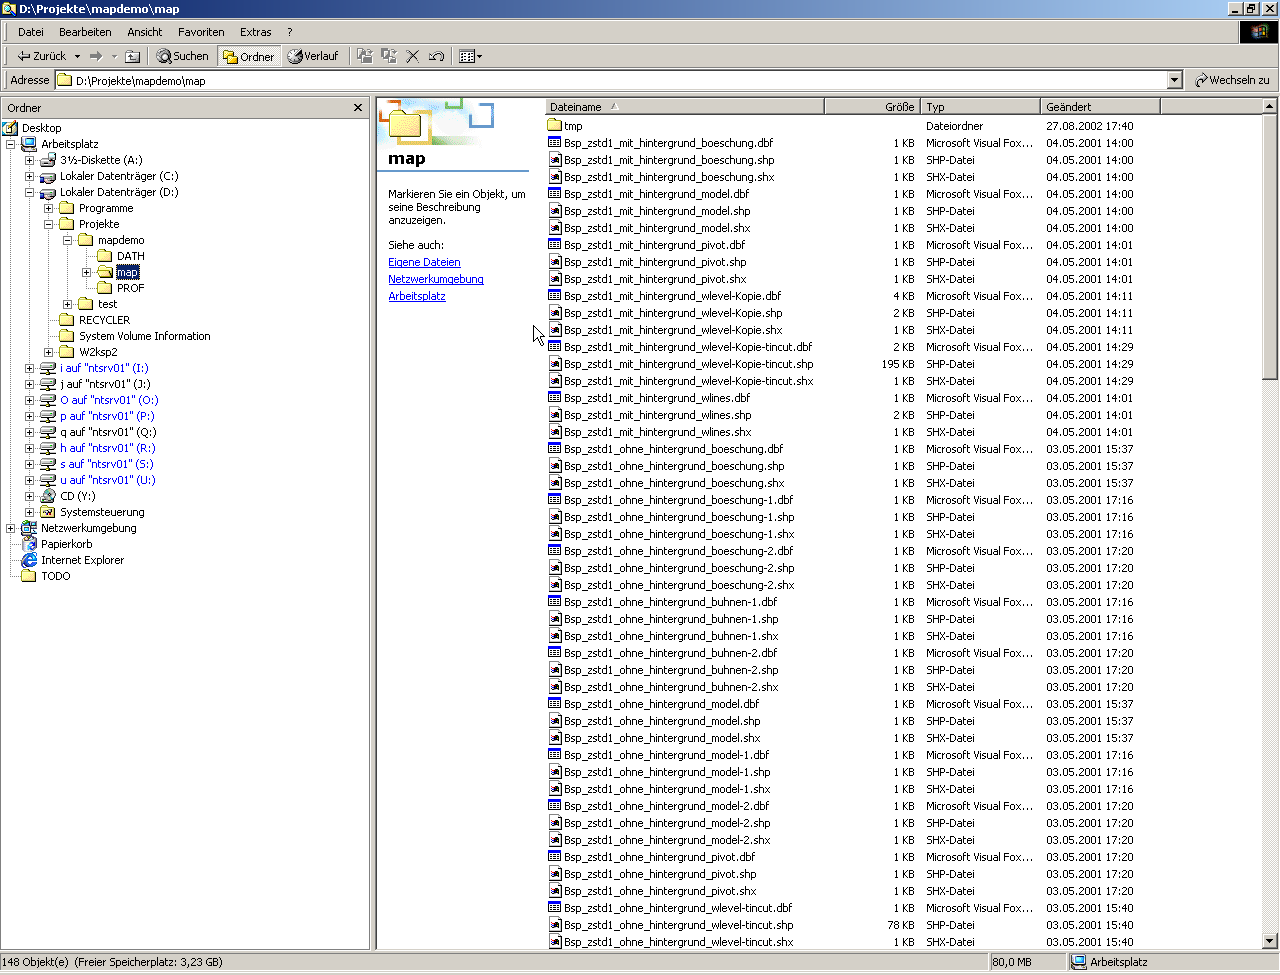
\includegraphics[scale=0.30]{abb25}
	\end{center}
	\caption{Speicherung von Themeninformationen}
	\label{fig:abb25}
\end{figure}
%Abb.25: Speicherung von Themeninformationen\\


\section{Geoobjekte bearbeiten}
\hypertarget{cmd:objekte-erzeugen}{}
\subsection{Objekt erzeugen}
\label{subsec:objekt-erzeugen}
Bevor ein neu angelegtes Thema bearbeitet werden kann, mu� zuerst 
ein Objekt erzeugt werden. Dazu wird  das entsprechende Thema (z.B. 'Trennfl�che/Neu')
in der �bersicht markiert und der Men�punkt \menu{Objekt erzeugen}gew�hlt (Abb. \ref{fig:abb9}).
\\

\begin{figure}[hbtp]
	\begin{center}
		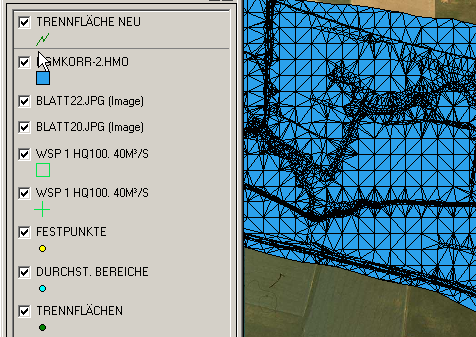
\includegraphics[scale=0.60]{abb9}
	\end{center}
	\caption{Geoobjekt (Trennfl�che/Neu) erzeugen}
	\label{fig:abb9}
\end{figure}
%Abb.9: Geoobjekt (Trennfl�chen-neu) erzeugen\\


Sobald man den Cursor in das Kartenfenster bewegt, wandelt sich dieser in einen Stift, mit
dem in der Karte ein neues Objekt des aktiven Themas digitalisiert werden kann. So wird z.B. jede Trennfl�chenposition mit einem Mausklick eingegeben. Die Eingabe von Linien oder Polygonen wird mit einem Doppelklick beendet. In der anschlie�enden Objektabfrage k�nnen dem neu erzeugten Objekt die entsprechenden Attribute zugewiesen werden.
Das neu angelegte Objekt kann auf vielf�ltige Weise bearbeitet und modifiziert werden.

\hypertarget{cmd:objekte-abfragen}{}
\subsection{Objektabfrage}
�ber die Men�folge \menu{Geo-Objekte / Objektabfrage} k�nnen die Attribute eines
Objektes jederzeit abgerufen und ver�ndert werden. Es erscheint ein Fragezeichen, das man
auf ein entsprechendes Objekt positionieren kann, worauf dessen Eigenschaften angezeigt
werden (Abb. \ref{fig:abb10b}).\\

\begin{figure}[hbtp]
	\begin{center}
		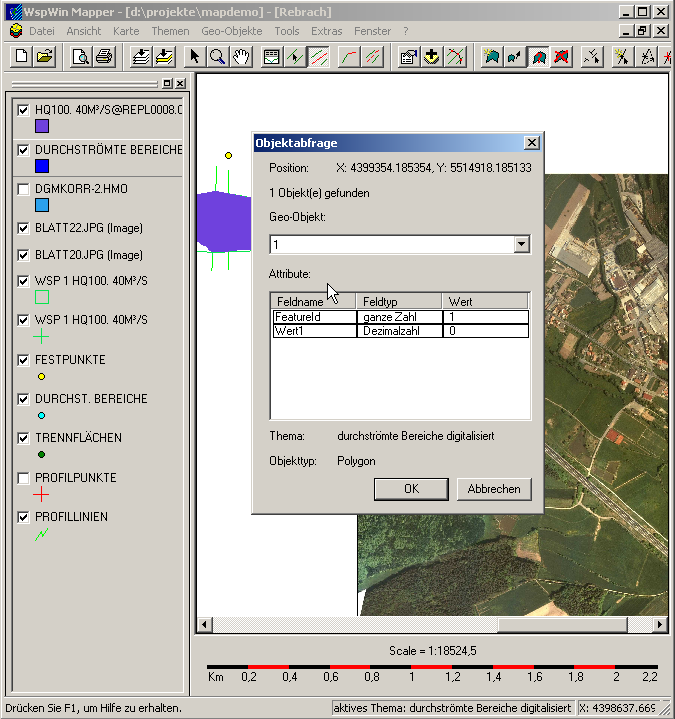
\includegraphics[scale=0.50]{abb10b}
	\end{center}
	\caption{Objektabfrage f�r Rauheitszone}
	\label{fig:abb10b}
\end{figure}
%Abb.10: Objektabfrage f�r Rauheitszone\\

\textbf{Hinweis:} Der Feldname und der Feldtyp des Objekts werden beim Erstellen des Objekts festgelegt und sind im Nachhinein nicht mehr ver�nderbar. Bei der Objektabfrage kann lediglich der Wert des Objektes ge�ndert werden. 

\hypertarget{cmd:objekte-verschieben}{}
\subsection{Objekt verschieben}
�ber die Men�folge \menu{Geo-Objekte / Objekt verschieben} l��t sich der
Verschiebemodus aktivieren. Ein Objekt (Punkt, Linie oder Vieleck) eines markierten
Themas kann dann bei gedr�ckter linker Maustaste an eine beliebige Stelle in der Karte
verschoben werden (Abb. \ref{fig:abb11}). Diese Option kann beispielsweise die Verschiebung der
Wasserspiegellinien vor dem Verschneiden mit einem DGM genutzt werden .\\

\begin{figure}[hbtp]
	\begin{center}
		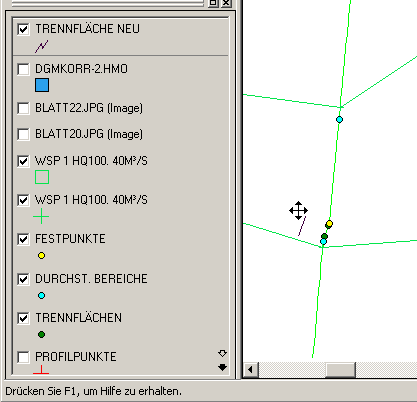
\includegraphics[scale=0.70]{abb11}
	\end{center}
	\caption{Parallelverschieben eines Trennfl�chenobjektes}
	\label{fig:abb11}
\end{figure}
%Abb.11: Parallelverschieben des neuen Trennfl�chenobjektes\\

\hypertarget{cmd:objekte-ausschneiden}{}
\subsection{Objekt ausschneiden}
�hnlich dem Verschieben eines Objektes kann ein Objekt auch kopiert werden, wobei es
m�glich ist, auch nur einen Teil des Objektes auszuschneiden, zu kopieren und an einer anderen Stelle einzuf�gen. Markieren Sie hierzu ein Thema, klicken Sie auf \menu{Geo-Objekte / Objekt ausschneiden} und markieren Sie �ber ein Polygon mit der Maus den betreffenden Ausschnitt in der Karte. Beendet wird der Vorgang durch einen Doppelklick. Nun haben Sie den betreffenden Ausschnitt kopiert und k�nnen ihn mit der Maus an einer beliebigen Stelle in der Karte wieder einf�gen (einmal Klicken).

\hypertarget{cmd:objekte-loeschen}{}
\subsection{Objekt l�schen}
Um ein Objekt aus der Darstellung zu l�schen, muss der L�schmodus aktiviert werden und im
selektiertem Thema das entsprechende Objekt mit einem Mausklick gel�scht werden.

\hypertarget{cmd:objekte-punkt-einfuegen}{}
\hypertarget{cmd:objekte-punkt-loeschen}{}
\hypertarget{cmd:objekte-punkt-verschieben}{}
\subsection{Punkt einf�gen, l�schen, verschieben}
In einem Linien- oder Polygon-Thema k�nnen Punkte 
hinzugef�gt, gel�scht oder verschoben werden. Dazu ist der entsprechende Modus aus dem
Men� \menu{Geo-Objekte} (z.B. \menu{Geo-Objekte / Punkt einf�gen} zu w�hlen. 

Folgende Optionen sind w�hlbar:\\
\menu{Punkt einf�gen}: Mit dem Stift an der Einf�geposition klicken und Maustaste gedr�ckt halten. Dem Geo-Objekt wird ein weiterer Punkt hinzugef�gt. Bei gedr�ckter Taste kann der eingef�gte Punkt verschoben werden.
\\
\menu{Punkt l�schen}: Durch Klick mit linker Maustaste k�nnen einzelne Punkte eines Geo-Objektes gel�scht werden.
\\
\menu{Punkt verschieben}: vorhandene Punkte eines Geo-Objektes k�nnen bei gedr�ckter linker Maustaste verschoben werden.
\\
Anm.: Bei Punkte-Themen m�ssen die vorhandenen Elemente (Punkte) �ber das Men� \menu{Geo-Objekte / Punkt verschieben (...l�schen)} bearbeitet werden.	

\section{Ausgabem�glichkeiten}

\hypertarget{cmd:datei-drucken}{}
\hypertarget{cmd:datei-seitenansicht}{}
\hypertarget{cmd:datei-druckereinrichtung}{}
\subsection{Drucken}

Erstellte Karten k�nnen auf einem Drucker /
Plotter zu Papier gebracht werden. Die Druckerauswahl sowie die Drucker-Einstellungen erfolgen �ber den Men�punkt \menu{Druckereinrichtung} im Dateimen� (Abb. \ref{fig:seitenansicht}). 
In der Seitenansicht besteht die M�glichkeit, die Formatierung und Anordnung der dargestellten Elemente zu ver�ndern.\\
\\
\begin{figure}[hbtp]
	\begin{center}
		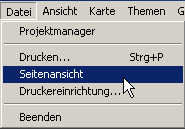
\includegraphics[scale=0.60]{seitenansicht}
	\end{center}
	\caption{Auswahl der Seitenansicht}
	\label{fig:seitenansicht}
\end{figure}


Elemente, die im Layout verf�gbar sind:
\begin{itemize}
	\item{Karte}
	\item{Projekt�berschrift}
	\item{Legende}
	\item{Textfeld}
	\item{Logo}
\end{itemize}

\begin{figure}[hbtp]
	\begin{center}
		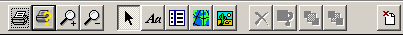
\includegraphics[scale=0.50]{toolleiste}
	\end{center}
	\caption{verf�gbare Aktionsbuttons f�r die Layoutgestaltung}
	\label{fig:toolleiste}
\end{figure}

In der Seitenansicht k�nnen diese Elemente hinzugef�gt, ge�ndert oder wieder entfernt werden. Dies betrifft sowohl die Projekt�berschrift (Abb.~\ref{fig:texteigenschaften}) als auch die Legende (Abb.~\ref{fig:legendeeigenschaften}). Das Element "`Firmenlogo"' (Abb.~\ref{fig:logofestlegen}) dient zur Platzierung einer Grafik-Datei im bitmap-Format z.B. im Zusammenhang mit einem Firmenstempel. Bei Textfeldern k�nnen Sie beliebigen Absatz-Text eingeben und diesen entsprechend formatieren (Abb.~\ref{fig:toolleiste}).
In der Legende werden nur die im Kartenfenster als sichtbar markierten Themen angezeigt. Um Themen  im Plot hinzuzuf�gen oder zu entfernen, m�ssen diese zun�chst in der Kartenansicht aktiviert bzw. deaktiviert werden.\\


\begin{figure}[hbtp]
	\begin{center}
		\includegraphics[scale=0.60]{legendeeigenschaften}
	\end{center}
	\caption{�ndern der Legende}
	\label{fig:legendeeigenschaften}
\end{figure}

\begin{figure}[hbtp]
	\begin{center}
		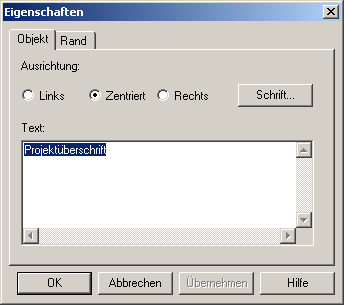
\includegraphics[scale=0.50]{texteigenschaften}
	\end{center}
	\caption{Texte eingeben oder �ndern}
	\label{fig:texteigenschaften}
\end{figure}

\begin{figure}[hbtp]
	\begin{center}
		
\includegraphics[scale=0.50]{logo}
	\end{center}
	\caption{Logo festlegen}
	\label{fig:logofestlegen}
\end{figure}


\subsubsection{Ausgabema�stab festlegen}
Die �nderung des Ausgabe-Ma�stabes ist mittels eines Doppelklicks auf das Kartenelement m�glich. Hier bestehen 2 Optionen:\\


\paragraph{Kartenausschnitt anpassen:}
\label{sec:KartenausschnittAnpassen}
Sie k�nnen den Kartenausschnitt an den neuen Ma�stab anpassen, d.h. es wird nur die Darstellung innerhalb des Kartenelemts gem�ss des von Ihnen gew�hlten Ma�stabs ge�ndert; die Gr��e des Kartenelemts selbst wird beibehalten.

\paragraph{Druckbereich anpassen:}
\label{sec:DruckbereichAnpassen}
\ In diesem Fall wird das Kartenelement und dementsprechend auch der Druckbereich an den vorgegebenen Ma�stab angepasst und erm�glicht z.B. eine ma�stabsgetreue Ausgabe im Grossformat
oder auf mehreren Ausgabebl�ttern.

\begin{figure}[hbtp]
	\begin{center}
		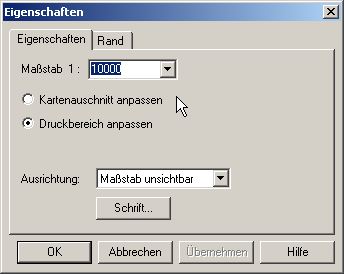
\includegraphics[scale=0.50]{massstab}
	\end{center}
	\caption{Ma�stab w�hlen}
	\label{fig:massstab}
\end{figure}

\begin{figure}[hbtp]
	\begin{center}
% KAPUTT!
%		\includegraphics[scale=0.40]{ausgabemoeg_preview}
	\end{center}
	\caption{Seitenansicht des Kartenfensters}
	\label{fig:ausgabemoeg_preview}
\end{figure}
%Abb.24: Seitenansicht des Kartenfensters\\

Zur Ausgabe der Karte dient das Druckersymbol. Die Karte wird mit den
vorgegebenen Druckereinstellungen - wie aus anderen Windows-Anwendungen
gewohnt - gedruckt.

\hypertarget{cmd:karte-exportierenals}{}
\hypertarget{cmd:karte-inzwischenablage}{}
\subsection{Bild speichern}
Im \wspmap\ besteht die M�glichkeit, die auf dem Bildschirm dargestellte Karte entweder als Bitmap (*.bmp) oder als EMF-Bilddatei (*.emf) zu exportieren \menu{Karte / Exportieren als}. Damit steht die erzeugte Karte f�r die Weiterverarbeitung mit anderen Anwendungen oder zur Einbindung in ein Text-Dokument zur Verf�gung.  

\section{Fortgeschrittene Handhabung}

\hypertarget{cmd:extras-nutzungsklassen}{}
\subsection{Zuweisen von Nutzungsklassen}
\wspmap\ bietet eine komfortable M�glichkeit, Profilen mit Hilfe von digitalen Landnutzungs-Themen Rauheiten und Bewuchs-Parameter zuzuordnen. F�r diese Option werden folgende Daten ben�tigt:\\
- Querprofile als Punkte-Thema (z.B. automatisch erzeugte Profilpunkte)\\
- digitalisierte Landnutzung als Polygon-Thema\\
- Nutzungstabelle, �ber die eine Zuordnung zwischen der Landnutzung und den dazugeh�rigen Parametern
  erfolgt\\
  \\

�ber die Men�folge \menu{Extras / Nutzungklassen} haben Sie die M�g\-lich\-keit, Rauheits- und
Bewuchswerte den Punkten der Querprofile zuzuordnen. Andererseits k�nnen Nutzungsklassen mit
verschiedenen Landnutzungsformen angelegt, diesen Werte zugeordnet und schlie�lich mit
Attributen (Einzelwerten) von z.B. importierten digitalisierten Landnutzungskarten im
shape-Format verschnitten werden. Dazu wird �ber \menu{Neu} ein Name f�r die Tabelle vergeben
und f�r jede 
Nutzungsart eine Zeile angelegt. �ber \ctrl{Spalte l�schen} und \ctrl{Neue Spalte} legen Sie
fest, welche Parameter zugeordnet werden sollen (Vermeiden Sie Werte mit 0 und l�schen Sie
besser die entsprechenden Spalten) (Abb. \ref{fig:abb16}). 
Die Tabellen werden in Ihrem Betriebssystemverzeichnis
im Unterverzeichnis \file{Wsp-Nutzklassen} einzeln gespeichert und k�nnen hier auch verwaltet
werden.\\

\begin{figure}[hbtp]
	\begin{center}
		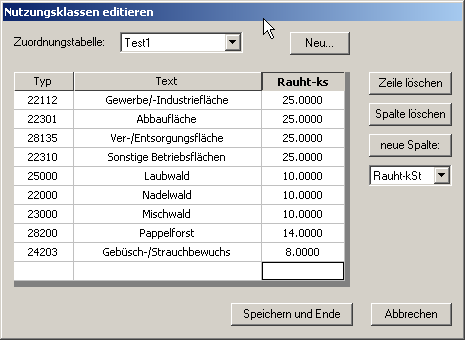
\includegraphics[scale=0.70]{abb16}
	\end{center}
	\caption{Anlegen von Nutzungsklassen}
	\label{fig:abb16}
\end{figure}
%Abb. 16: Anlegen von Nutzungsklassen

\hypertarget{cmd:themen-mitprofilenschneiden}{}
\subsection{Objekte mit Profilen schneiden}
Es mu� zun�chst entschieden werden, ob Nutzungsklassen zuzuordnen sind (bei den
Datens�tzen Rauheit ks, kSt sowie Bewuchs AX, AY, DP) oder Trennlinien (bei Trennfl�chen
und Durchstr�mten Bereichen) erzeugt werden sollen. Im Fall der Nutzungsklassen mu� eine
Tabelle zugeordnet werden und festgelegt werden, welchem Attribut diese zuzuordnen ist (Abb. \ref{fig:abb13}).\\

\begin{figure}[hbtp]
	\begin{center}
		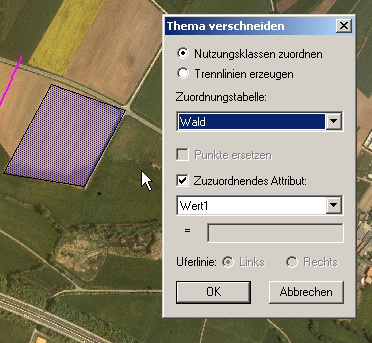
\includegraphics[scale=0.70]{abb13}
	\end{center}
	\caption{Thema mit Profil verschneiden �ber Nutzungsklassen}
	\label{fig:abb13}
\end{figure}
%Abb.13: Thema mit Profil verschneiden �ber Nutzungsklassen\\
Im Fall der Trennlinien ist das zu erstellende Thema zu w�hlen und festzulegen, ob evtl.
vorhandene Trennlinien ersetzt werden sollen. Gegebenenfalls ist eine Einschr�nkung auf ein
bestimmtes Attribut m�glich  (Abb. \ref{fig:abb14}).\\

\begin{figure}[hbtp]
	\begin{center}
		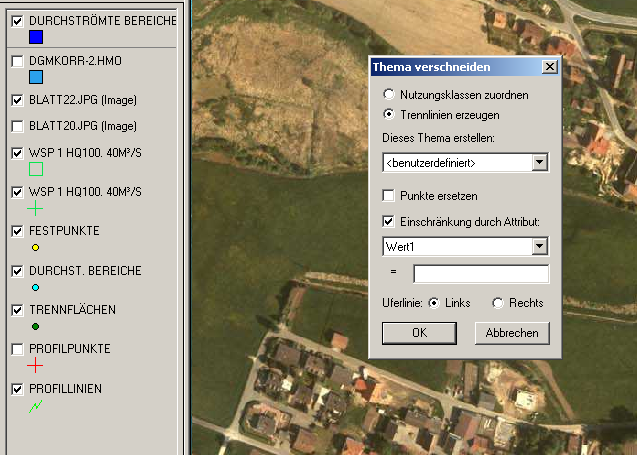
\includegraphics[scale=0.60]{abb14}
	\end{center}
	\caption{Thema mit Profil verschneiden f�r Trennlinien}
	\label{fig:abb14}
\end{figure}

%Abb.14: Thema mit Profil verschneiden f�r Trennlinien\\

Um ein neu angelegtes oder importiertes/hinzugef�gtes Thema auch \\ tats�chlich im Profil als
einen Punkt innerhalb der referenzierten Datens�tze zu speichern, muss das Linien- oder
Polygonthema (z.B. Trennfl�chen-neu) mit den Profilen verschnitten werden. Hierzu markiert
man das entsprechende Thema in der Themen�bersicht. Mit einem Klick auf die
rechte Maustaste erscheint das Kontextmen� und es wird \menu{Mit Profilen schneiden}
ausgew�hlt. Nachdem die Verschneidung durchgef�hrt wurde, sind die entsprechenden
Punkte in der Karte und im Querprofil ersichtlich. Sie werden in das ggf. bereits
existierende Thema integriert.


\hypertarget{cmd:profilabstaende-ermitteln}{}
\subsection{Ermittlung von Profilabst�nden}
Unter dem Men� \menu{Extras / Profilabst�nde ermitteln} werden die Abst�nde zwischen den Profilen auf Grundlage der Georeferenzierung neu berechnet. Zur Aktivierung des Men�punktes muss zun�chst das Thema \emph{Profillinien} aktiviert werden. 

Die Abstandsberechnung erfolgt jeweils automatisch zwischen zwei aufeinander folgenden Profilen f�r das Hauptgerinne, das linke und rechte Vorland. Die Profilabst�nde werden anschlie�end in einer Tabelle auf dem Bildschirm ausgegeben (Abb.~\ref{fig:profilabstaende}).

\begin{figure}[hbtp]
	\begin{center}
		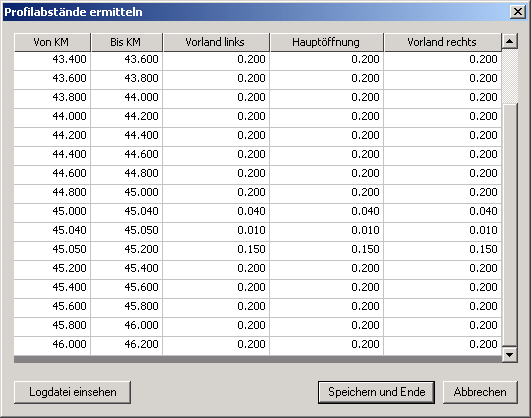
\includegraphics[scale=0.60]{profilabstand}
	\end{center}
	\caption{Ausgabetabelle nach Ermittlung der Profilabst�nde}
	\label{fig:profilabstaende}
\end{figure}

�ber die Schaltfl�che \menu{Speichern und Ende} werden die aktuell ermittelten Abst�nde in die Strangtabelle des WSPWIN-Projektes (nach erneuter Best�tigung) �bernommen. Durch Klick auf \menu{Abbrechen} wird die Tabelle geschlossen. Zus�tzlich kann auch die Logdatei als Text eingesehen werden.

\hypertarget{cmd:flip-profiles}{}
\subsection{Profile Spiegeln}
Der Men�punkt \menu{Tools / Profil spiegeln} erm�glicht das Spiegeln der Profilpunkte mit der Mittelachse als Spiegellinie. Nach Aktivierung des Tools erfolgt  die Spiegelung eines Profils durch Klick mit dem Stiftsymbol auf eine Profillinie. Die �berpr�fung des Ergebnisses kann durch Visualisierung in der Profilansicht erfolgen.

Die Profilspiegelung wird zun�chst nur in der Kartenansicht gespeichert. Sollen die �nderungen in das Berechnungsprogramm WspWin �bertragen werden, m�ssen die entsprechenden Querprofile �ber die Profil�bersicht gespeichert werden (vgl. auch Abschnitt~\ref{subsec:profildaten-speichern}). 
	
\hypertarget{cmd:themen-Hoehenmodellimportieren}{}
\section{Arbeiten mit digitalen H�henmodellen}
Um Pre- und Postprocessing in \wspmap\ anhand von digitalisierten H�hendaten durchf�hren zu k�nnen, besteht die M�glichkeit digitale Gel�ndemodelle (DGMs) in eine Karte zu importieren. Mit einem importierten Gel�ndemodell k�nnen die folgenden Operationen durchgef�hrt werden:
\begin{itemize}
	\item Generieren von Querprofilen
	\item Verl�ngern von Querprofilen
	\item Ermitteln von �berflutungsfl�chen anhand gerechneter Wasserspiegel
	\item Fliesstiefendarstellungen anhand gerechneter Wasserspiegel
\end{itemize}

\subsection{Importieren von Gel�ndemodellen}
Bevor Daten aus Gel�ndemodellen zur Bearbeitung der Projektdaten herangezogen werden k�nnen, muss ein Gel�ndemodell in die Karte eingelesen werden.
\wspmap\ bietet die Option sowohl bereits vermaschte H�henmodelle zu importieren als auch reine Punktdaten zu laden und diese zu triangulieren.

\begin{figure}[hbtp]
	\begin{center}
		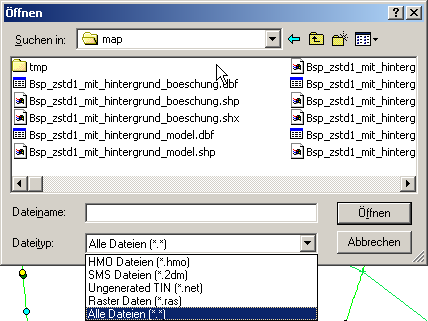
\includegraphics[scale=0.70]{abb27}
	\end{center}
	\caption{H�henmodellimport}
	\label{fig:abb27}
\end{figure}

\wspmap\ kann die folgenden Formate als Gel�ndemodell importieren:
\begin{itemize}
	\item *.hmo: BCE-eigenes H�henmodell-Format HMO
  \item *.2dm: SMS-Format (Surfacewater Modeling Software oder �ber GeoCADOP)
	\item *.net: 'ungenerated tin' - Format ESRI ArcINFO
	\item *.ras: reine Punktdaten (Rechtswert, Hochwert, H�he)
\end{itemize}

Beispieldateien f�r alle genannten Daten befinden sich auf der Installations-CD.

Erkennt das Programm beim Import, dass keine Vermaschung vorliegt wird der Benutzer gefragt, ob die Punktdaten vermascht werden sollen. 

Sind die Daten bereits trianguliert wird die vorhandenen Vermaschung �bernommen und  vorhandene Bruchkanten bleiben erhalten.

Nach dem Import eines H�henmodells wird automatisch ein Thema f�r das DGM angelegt
und im Kartenausschnitt dargestellt (siehe Abb.~\ref{fig:imported-dgm}).

\begin{figure}[hbtp]
	\begin{center}
		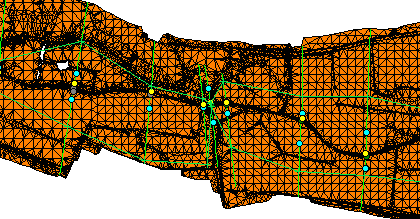
\includegraphics[scale=1.0]{dgm}
	\end{center}
	\caption{Importiertes H�henmodell}
	\label{fig:imported-dgm}
\end{figure}
%Abb.27: H�henmodellimport\\

\hypertarget{cmd:tools-profilgenerieren}{}
\subsection{Querprofile erzeugen}
\wspmap\ bietet die M�glichkeit, anhand eines importierten H�hen\-modells neue
Profile in einem Projekt zu generieren.

W�hlen Sie hierzu den Men�punkt \menu{Tools / Profil generieren} oder das entsprechende Symbol aus der Symbolleiste. Das Tool kann nur aktiviert werden, wenn ein H�henmodell importiert wurde.\\

Voraussetzung f�r die Erzeugung neuer Profile aus einem digitalen H�hen\-modell ist das Vorhandensein einer Flussachse.
Die Flussachse ist zur Ermittlung der Stationierung und Profilabst�nde
bzw. zur Einsortierung in die Strangtabelle erforderlich. Sie sollte mindestens die beiden
benachbarten Profile des neu zu generierenden Profils schneiden und im Allgemeinen in der
Flu�mitte liegen. Die Flussachse darf jedes Profil h�chstens einmal schneiden. 

\subsubsection{Erzeugen einer Flussachse}
Nach Aktivierung des Men�punktes bzw. des entsprechenden Symbols folgt, sofern noch
keine Flussachse vorhanden ist, ein Hinweis, dass zun�chst eine Hilfslinie in L�ngsrichtung des Gew�ssers zu zeichnen ist. Durch Klicken auf die Karte kann die Flussachse direkt digitalisiert werden, �hnlich wie dies beim Erzeugen von Objekten eines Linienthemas geschieht (siehe Abschnitt \ref{subsec:objekt-erzeugen}). Der Benutzer
hat die M�glichkeit, den Vorgang durch Dr�cken der Escape-Taste abzubrechen. Durch
Doppelklick wird die Linie fertiggestellt. Sie wird dann als gestrichelte blaue Linie
dargestellt. Wenn die Linie sp�ter nicht mehr ben�tigt wird oder eine neue Linie gezeichnet
werden soll, kann die vorhandene mittels ESC gel�scht werden. 

Wird eine Flussachse mehrfach ben�tigt, kann man ein entsprechendes Thema anlegen. Dazu erzeugt man entweder ein neues Linienthema (wie in Abschnitt \ref{subsec:thema-erzeugen} beschrieben) oder importiert ein bereits vorhandenes (siehe Abschnitt \ref{subsec:thema-einfuegen}). In beiden F�llen muss gew�hrleistet sein, dass ein Attribut 'VZK' vorhanden ist. Das Attibut 'VZK' muss dabei als \emph{ganze Zahl} bzw. als Integer definiert sein, um vom Programm erkannt zu werden. Das Attribut dient bei verzweigten System zur Zuordnung der Verzweigungskennung und sollte bei unverzweigten System konstant 0 sein.
Dieses Thema kann nun durch einfaches Kopieren zur Flussachse umdefiniert werden. W�hlen Sie beim Kopieren des Themas (Men�punkt \menu{Thema/Kopieren}) als Typ des neuen Themas 'Flussachse'.

\subsubsection{Ein einzelnes Profil generieren}
Falls eine Flussachse existiert, k�nnen beliebig viele Profile erzeugt werden.

Die neuen Profile werden durch direkte Eingabe der Lage in die Karte erzeugt (\menu{Tools / Profil generieren}). Dies erfolgt durch Zeichnen einer Linie in der Karte. Auch hier wird mit Escape abgebrochen und durch Doppelklick die Eingabe abgeschlossen. Die neue Profil-Linie mu� die Flussachse schneiden.\\
Weiterhin ist darauf zu achten, die Profile in Fliessrichtung von links nach rechts zu digitalisieren, da die neuen Profilpunkte in Richtung der digitalisierten Linie in das Profil einsortiert werden.

Nachdem die Profillinie erstellt worden ist, wird sie mit dem Gel�ndemodell verschnitten. Der Benutzer erh�lt eine Vorschau des Profils sowie Angaben �ber die benachbarten Profile, die der Stationierung, Abstandsberechnung und Kilometrierung zugrunde gelegt werden. Ferner
mu� der Zustand selektiert werden, in den das Profil einzusortieren ist. Die vorgeschlagenen Daten k�nnen bei Bedarf korrigiert werden. Sobald 'Profil hinzuf�gen' gew�hlt ist, wird das Profil gespeichert und direkt in die Strangtabelle einsortiert.

\begin{figure}[hbtp]
	\begin{center}
		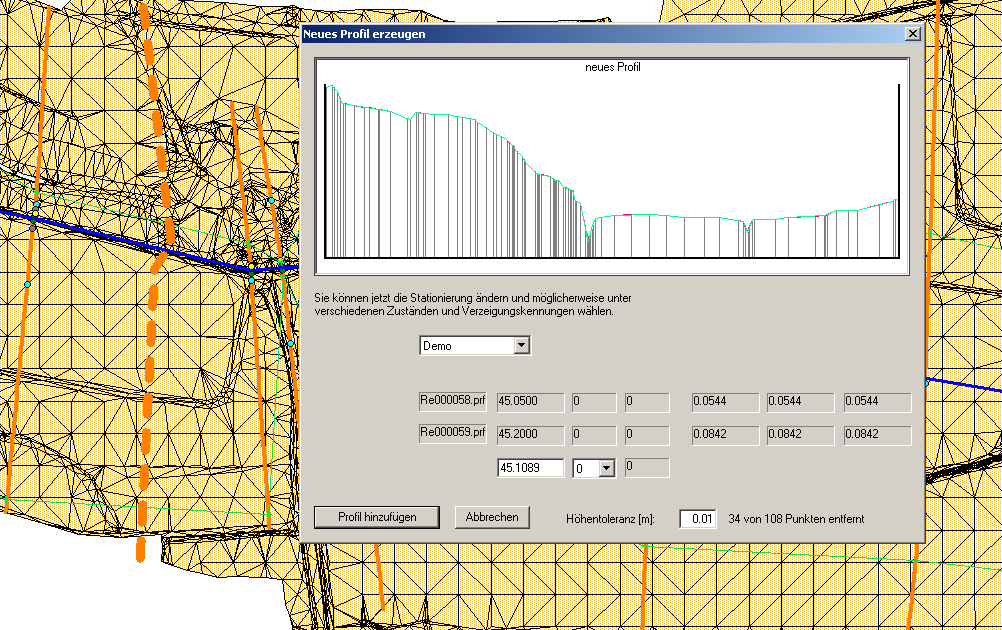
\includegraphics[scale=0.35]{genprof}
	\end{center}
	\caption{Erzeugen und Einf�gen eines neuen Profils}
	\label{fig:genprof}
\end{figure}

\paragraph{Profildaten ausd�nnen}
Der Algorithmus zum Auslesen der Gel�ndedaten aus dem digitalen Gel�ndemodell produziert alle Schnittpunkte entlang der digitalisierten Profillage. Dies f�hrt in vielen F�llen aber zu einer grossen Zahl von H�henpunkten, die der gew�hlten Aufgabenstellung nicht entsprechen und in der sp�teren Bearbeitung hinderlich sein k�nnen.\\
Aus diesem Grunde wurde die Maske zur Voransicht des generierten Profils erweitert, um nicht-relevante Profilpunkte automatisch auszusortieren. Im Diagramm wird die urspr�nglich ausgelesene Profillinie rot, die ausged�nnte gr�n dargestellt. Der Benutzer kann die (standardm�ssig auf 1cm eingestellte) max. H�hentoleranz einstellen, um das Ergebnis zu optimeren. Bei jeder �nderung der H�hentoleranz wird die gr�ne Profilgeometry neu gezeichnet.

\subsubsection{Mehrere Profile automatisch generieren}
Alternativ k�nnen mehrere Profile automatisiert mit Hilfe eines beliebigen Linienthemas erzeugt werden, welches die Lage der Profile beschreibt (\menu{Tools / Profile generieren}). Alle Objekte des Themas werden mit dem Gel�ndemodell verschnitten und zu einem (vorher auszuw�hlenden) Zustand hinzugef�gt. Bei jeder verschnittenen Profillage erscheint der gleiche Dialog wie beim einzelnen generieren einzelner Profile.\\
Ist im Linienthema zus�tzlich das Attribut 'Station' als Dezimalzahl vorhanden. Wird die Station automatisch f�r die neuen Profile �bernommen, der Dialog 'Profil generieren' entf�llt in diesem Fall.

\hypertarget{cmd:tools-profilverlaengern}{}
\subsection{Querpfofile verl�ngern}

\begin{figure}[hbtp]
	\begin{center}
		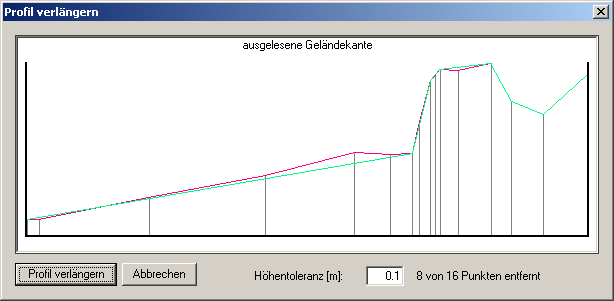
\includegraphics[scale=0.60]{extendprofile}
	\end{center}
	\caption{Einf�gen einer Profilverl�ngerung}
	\label{fig:extendprofile}
\end{figure}

Neben dem Generieren neuer Profile besteht auch die M�glichkeit, bestehende Profile zu
verl�ngern. H�ufiger Anwendungsfall ist die Verl�ngerung terrestrisch gemessener Profile (z.B: Vermessung des Flussschlauchs per Echolot) �ber das Vorland hinaus anhand von Gel�ndedaten aus �berfliegungen.\\
Nach Wahl des Men�punktes \menu{Tools / Profil verl�ngern} muss der Endpunkt eines vorhandenen Profiles ausgew�hlt werden. Die Profilverl�ngerung kann durch wiederholtes Klicken auf die Karte digitallisiert werden. Ein Doppelklick schliesst die Eingabe ab. Das Profil wird dabei bis zum ersten St�tzpunkt geradlinig fortgesetzt, ist dies nicht gew�nscht l�st ein Druck auf Escape die Richtungsvorgabe. Ein zweites Dr�cken der Escape-Taste bricht den Vorgang ab.\\
Nach Abschluss der Eingabe erscheint ein �hnlicher Dialog wie beim Generieren von Profilen, die Eingabe der Querprofildaten (z.B. Station) entf�llt hier nat�rlich. 
Wie bei 'Profil generieren' ist aber auch hier das Ausd�nnen der Profildaten m�glich.\\
Nach Best�tigung des Dialogs wird das Profil in der Karte verl�ngert und kann in der Profilansicht eingesehen werden. Die �nderungen des Profils werden allerdings im Gegensatz zum 'Profil generieren' erst in die Profildatei �bertragen, nachdem die Bearbeitung gespeichert wurde (Diskettensymbol im Dialog 'Profilauswahl').

\hypertarget{cmd:themen-dgmmitwasserspiegel}{}
\subsection{Ausweisung von �berflutungsfl�chen}
Mit Hilfe von  \wspmap\ ist es m�glich, berechnete Wasserspiegellagen im Lageplan als �berflutungsfl�chen zu visualisieren.

Um die Wasserspiegellagen in die Karte zu laden, m�ssen diese in den Querprofilen eingetragen sein. Dies geschieht zum einen nach jeder Rechnung (nur die gerechneten Berechnungsvarianten) oder kann im Projektmanager im Men� \menu{L�ngsschnitt / Wsp einf�gen in Querprofile} nachtr�glich durchgef�hrt werden.

Sind die Wasserspiegel in den Querprofilen eingetragen, werden diese beim (Neu-)einladen der Querprofile automatisch als Themen im Lageplan angelegt. Pro gerechnetem Wasserspiegel wird dabei ein Punkt-Thema der Durchstichpunkte des Wasserspiegels im Querprofil und ein Polygon-Thema (Linear-verbundene Wasserspiegel) erzeugt. Die Themen werden analog der Berechnungsvariante benannt.

Das neu erzeugte Polygon-Thema kann bereits zum Ausweisen von �ber\-schwemmungs\-fl�chen herangezogen werden, die das Relief eines unterliegenden Gel�ndemodells wird dabei aber nicht ber�cksichtigt (siehe Abb.~\ref{fig:wsp-linear}).

\begin{figure}[hbtp]
	\begin{center}
		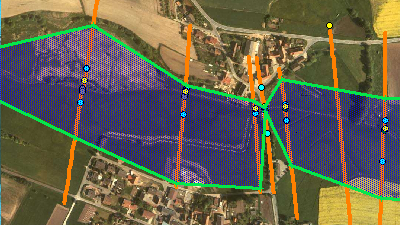
\includegraphics[scale=1.0]{wsp-linear}
	\end{center}
	\caption{lineare Darstellung der gerechneten Wasserspiegel}
	\label{fig:wsp-linear}
\end{figure}

\subsection{Verschneidung der WSP-Lagen mit einem DGM}
\label{sec:dgm:tincut}
Um die zus�tzliche Gel�ndeinformation eines digitalen Gel�ndemodells auszunutzen, ist es �ber die lineare Darstellung der �berflutungsfl�chen hinaus m�glich, diese mit einem DGM zu verschneiden, um z.B. Einbuchtungen oder Ausuferungen zwischen den Profilen darstellen zu k�nnen.

Die Verschneidung wird �ber den Men�punkt \menu{Themen / mit H�henmodell verschneiden} ausgel�st, wobei das zu verschneidende Thema ausgew�hlt sein muss (das Punktthema).

Nach Auswahl des Men�s wird die externe Anwendung 'Fliesstiefenermittlung' gestartet, welche die eigentliche Verschneidung durchf�hrt. Im Fall der Ausweisung von �berflutungsfl�chen kann hier nur die Genauigkeit der Verschneidung eingestellt werden, wobei eine Gr�sse von kleiner als 1[m] im allgemeinen nicht sinvoll ist und die Rechenzeit erheblich beinflussen kann.

Nach Start der Verschneidung mit 'Ok' wird der Fortschritt der Operation angezeigt und danach das Ergebnis automatisch als neues Thema eingeladen.

\paragraph{Arbeitsweise des Verschneidungsalgorythmus}
\ \\Die Verschneidung der Wasserspiegellagen und dem ausgew�hlten DGM erfolgt rein geometrisch, es werden keine hydraulischen Begebenheiten ber�cksichtigt. Zu diesem Zweck wird aus den Wasserspiegelh�hen an den Querprofilen ein digitales H�henmodell der Wasserspiegeloberfl�che generiert. Der Verschneidungsalgorythmus ermittelt nun die Auftragsfl�chen dieses H�henmodells �ber dem Gel�ndemodell und generiert ein entsprechenden Polygonthema. Dabei wird im ersten Schritt lediglich die durch die lineare Verbindung der Wasserspiegellagen umrandete Fl�che ber�cksichtigt.

\paragraph{Extrapolation der Wasserspiegellagen}
\ \\Um die zu verschneidende Fl�che zu vergr�ssern besteht die M�glichkeit, diese manuell festzulegen. Dazu muss als erstes das Punktthema der zu bearbeitenden Wasserspiegellage kopiert werden. Wird das kopierte Thema ausgew�hlt, wird die zu verschneidende Fl�che als Umrandung in der Karte dargestellt. Das Punktthema kann jetzt wie jedes andere Profilbezogene Thema (z.B: Trennfl�chen) auf den Profillinien verschoeben werden, die Umrandung wird dabei nachgef�hrt. Zur Vereinfachung der Bearbeitung kann der Men�punkt \menu{Themen / Wasserspiegel nach aussen setzen} gew�hlt werden, um die Umrandung auf die Profilenden zu setzen.

Wird jetzt der Befehl \menu{mit H�henmodell verschneiden} auf dem Bearbeiteten Thema ausgef�hrt, wird die erweiterte Fl�che zur Verschneidung herangezogen (siehe Abb.~\ref{fig:tincut}).

\begin{figure}[hbtp]
	\begin{center}
		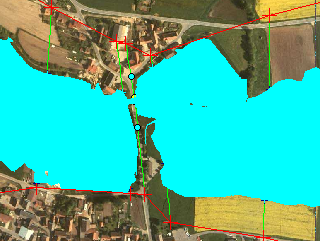
\includegraphics{tincut}
	\end{center}
	\caption{aus der Verschneidung mit extrapoliertem WSP berechnetes �berschwemmungsgebiet}
	\label{fig:tincut}
\end{figure}

\subsection{Ermittlung von Flie�tiefen}
Neben dem Ausweisen der �berflutungsfl�che ist es auch m�glich, eine Fliesstiefendarstellung zu erzeugen\footnote{Diese Option ist nicht im normalen Lieferumfang von \wspmap\ enthalten}. Die Erzeugung der Flie�tiefendarstellung l�uft dabei identisch zur Erzeugung von �berflutungsfl�chen ab (siehe~\ref{sec:dgm:tincut}). 

Wurde die Flie�tiefenermittlung zus�tzlich erworben, besteht im Dialogfenster zur Erzeugung der Flie�tiefen die M�glichkeit, die Grenzen der Flie�tiefenermittlung auszuw�hlen (Abb.~\ref{fig:fliti-dlg}).

\begin{figure}[hbtp]
	\begin{center}
		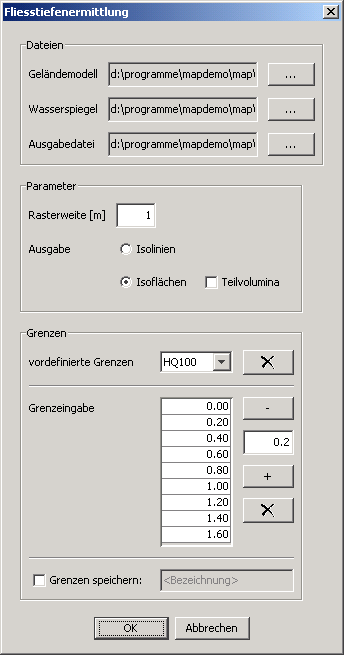
\includegraphics[scale=0.50]{fliti-dlg}
	\end{center}
	\caption{Eingabe der Bereichsgrenzen zur Flie�tiefenermittlung}
	\label{fig:fliti-dlg}
\end{figure}

Folgende Parameter sind vom Benutzer editierbar:

\emph{Dateien}:
Die zur Flie�tiefendarstellung notwendigen Dateien (H�henmodell, Wasserspiegel, Ausgabedatei im shape-Format) werden standardm��ig im aktuellen Projektverzeichnis abgelegt. Die Pfade k�nnen vom Benutzer beliebig ge�ndert werden. 

\emph{Parameter}:
F�r die vorgegebene Rasterweite werden die Flie�tiefen entweder als H�henlinien (Option 'Isolinien') oder als Bereich der Wasserspiegellage (Option 'Isofl�chen') ausgegeben. Die Rasterweite wird mit 1 m vorgegeben, was im Regelfall eine ausreichend detaillierte Flie�tiefendarstellung erzeugt. Sie kann jedoch beliebig vom Benutzer ge�ndert werden. Es gilt: Je kleiner die Rasterweite, desto detaillierter die Flie�tiefendarstellung (mit entsprechend l�ngerer Rechenzeit). 

Bei Aktivierung des K�stchens "Teilvolumina" erfolgt gleichzeitig mit der Flie�tiefenberechnung eine Ermittlung des Wasservolumens zwischen zwei Querprofilen. Diese Option verl�ngert die Rechendauer allerdings immens und sollte nur bei tats�chlichem Bedarf gew�hlt werden.

\emph{Grenzen}:
In diesem Dialogfeld werden die H�henintervalle f�r die Flie�tiefendarstellung vorgegeben. Dabei kann auf zuvor gespeicherte Intervall-Informationen zur�ckgegriffen oder die Intervalle per Hand eingegeben werden. Bei Bedarf k�nnen die eingegebenen Intervalle f�r eine erneute Benutzung gespeichert werden (H�kchen "Grenzen speichern" aktivieren und Bezeichnung eingeben).
Durch Vorgabe eines festen Intervalls kann �ber die Schaltfl�chen "+" und "-" die vorhanden Grenzen erweitert bzw. reduziert werden (siehe Beispiel in Abb.~\ref{fig:fliti-dlg}).

Durch Best�tigung auf "OK" wird die Berechnung zur Flie�tiefenermittlung gestartet. Die ermittelten Flie�tiefen werden anschlie�end der Karte als neues Thema hinzugef�gt und
nach vordefiniertem Farbverlauf eingef�rbt. Gleichzeitig �ffnet sich ein Dialogfenster, in dem das zu den Flie�tiefen geh�rige Gesamtvolumen als Information ausgegeben wird (Abb. \ref{fig:fliti-result}).

\begin{figure}[hbtp]
	\begin{center}
		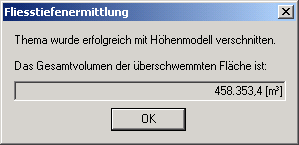
\includegraphics{fliti-result}
	\end{center}
	\caption{Ausgabe des Gesamtvolumens der �berschwemmten Fl�che}
	\label{fig:fliti-result}
\end{figure}

Die Darstellung des Flie�tiefen-Themas kann vom Benutzer wie bei einem Polygon-Thema ge�ndert werden.

Das erzeugte Thema wird als ESRI Shape-Datei im Projekt unter dem im Dialogfenster vorgegebenen Dateinamen abgelegt und kann mit anderen Programmen weiterverarbeitet werden. 

\begin{figure}[hbtp]
	\begin{center}
		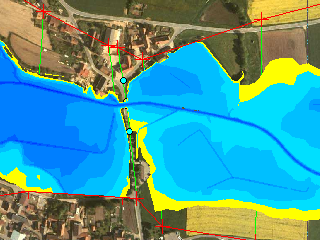
\includegraphics{fliesstiefen}
	\end{center}
	\caption{Ermittelte Fl�chen gleicher Flie�tiefe (Isofl�chen)}
	\label{fig:fliti}
\end{figure}



%\printindex
\listoffigures


\end{document}
